\documentclass{article}
\usepackage{graphicx} 
\usepackage{blindtext}
\usepackage[T1]{fontenc}
\usepackage{gensymb}
\usepackage{tikz}
\usepackage{multicol}
\usepackage{tabularx}
\usepackage{url}
\usepackage[a4paper, total={6in, 8in}]{geometry}
\usepackage{hyperref}

\begin{document}

\section{Imprint}
\begin{itemize}
    \item \textbf{Author:}~Filip Roučka
    \item \textbf{Institution:}~Czech Technical University in Prague, Faculty of Civil Engineering, Department of Geomatics
    \item \textbf{Subject:} 155PKAR
    \item \textbf{Date:} 18.05.2025
    \item \textbf{Coordinate system:} LAEA~[EPSG:3035]
\end{itemize}
Any items, data or graphics not found in this document were captured or created by the author.

\section{Data sources}
\begin{itemize}
    \item Light pollution \cite{eog_vnl_annual_v2}
    \item Europe \cite{eurostat_gisco_countries}
    \item Europe cities \cite{eurostat_urban_audit}
    \item Czech Republic \cite{arcgis_online_dataset}
    \item Czech Republic regions \cite{arcgis_online_dataset}
    \item Czech Republic region capitals \cite{arcgis_online_dataset}
    \item Observatories  \cite{wiki_astronomical_observatories}
    \item Astronomical installations \cite{rise_hvezd_mapotic}
\end{itemize}

\section{Infographics sources}
\subsection*{What is light pollution?}

Light pollution is the excessive or misdirected artificial light that brightens the night sky, reducing visibility of stars and disrupting natural ecosystems. It is caused by artificial sources such as streetlights, buildings, and signage that unnecessarily emit light upwards or stay illuminated. Light pollution not only affects astronomical observations but also impacts wildlife behaviour and human health by disturbing natural sleep cycles. Reducing it involves using properly shielded lighting and minimising unnecessary night-time illumination\cite{wiki_light_pollution}\cite{IDA_light_pollution}.

\subsection*{Data acquisition process?}

To accurately measure the brightness of the night sky (particularly in the context of light pollution studies), night-time satellite imagery of the Earth is used to capture the number and intensity of artificial light sources across the planet. The most important satellites collecting this data are those equipped with the VIIRS Day/Night Band (DNB) sensor\cite{wiki_light_pollution}\cite{eog_vnl_annual_v2}.\\
The raw data from these satellites is measured in radiance and is typically expressed in units of W\,m\textsuperscript{-2}\,sr\textsuperscript{-1} (watts per square metre per steradian). This unit indicates the amount of light energy emitted or reflected per unit area (m²) in a specific direction (solid angle in steradians). It is a physical measurement of emitted light power, independent of human perception\cite{wiki_light_pollution}\cite{wikipedia_radiance}.\\
The radiance measured in W\,m\textsuperscript{-2}\,sr\textsuperscript{-1} is useful for scientific analysis, while other units, such as candela per square metre (cd/m²) or magnitudes per square arcsecond (mag/arcsec²), are used to express how bright the sky appears to the human eye or how it affects astronomical visibility\cite{wiki_light_pollution}\cite{wikipedia_radiance}.

\subsection*{Total Solar Eclipse across Europe}

A total solar eclipse will occur on 12 August 2026, offering observers in Iceland, Spain and Portugal a rare opportunity to witness the Sun being fully covered by the moon. This will be the first such event since 1999\cite{wiki_2026_aug12_eclipse}\cite{timeanddate_2026_aug12_eclipse}.

\subsection*{How is a solar eclipse measured?}
Solar eclipses are most commonly measured in terms of magnitude, representing the fraction of the Sun's diameter obscured by the Moon, as seen from a given location. Values range from 0.0 to just over 1.0. We distinguish between the following types of eclipses\cite{timeanddate_eclipse_magnitude}:

\begin{itemize}
    \item \textbf{Partial Eclipse:} The Moon only covers part of the Sun's diameter\cite{timeanddate_eclipse_magnitude}.
    \item \textbf{Annular Eclipse:} The Moon appears smaller than the Sun, so it doesn't completely cover it. This leaves a ring of sunlight, known as an annulus, visible around the Moon\cite{timeanddate_eclipse_magnitude}.
    \item \textbf{Total Eclipse:} The Moon appears big enough to fully cover the Sun's bright circle\cite{timeanddate_eclipse_magnitude}.
\end{itemize}

\subsection*{Dark Sky Parks in the Czech Republic}

JOTO (Izera Dark Sky Park) is the first of its kind in the world. The park was officially declared on 4 November 2009, during the International Year of Astronomy. It extends across an area of 308 square kilometres in the Czech Republic and Poland\cite{astrocz_oblasti_tmave_oblohy}.\\
BOTO (Beskydy Dark-Sky Park) is the second International Dark Sky Park in the world. The park was officially declared on 4 March 2013. It extends across an area of 308 square kilometres in the Czech Republic and Slovakia\cite{astrocz_oblasti_tmave_oblohy}.\\
MOTO (Manětín Dark Sky Park) is the first park completely in the Czech Republic. The park was officially declared on 15 September 2014. It covers an area of 346 square kilometres\cite{astrocz_oblasti_tmave_oblohy}.

\section{Image sources}
\noindent
\begin{minipage}[t]{0.1\textwidth}
    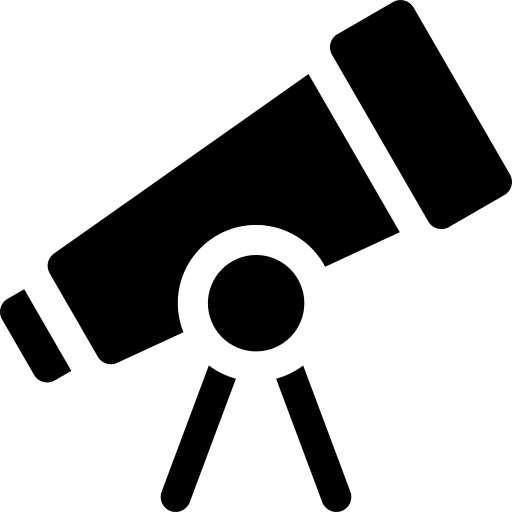
\includegraphics[width=\linewidth]{Image/telescope.png}
\end{minipage}
\hfill
\begin{minipage}[t]{0.85\textwidth}
    Telescope icon \cite{flaticon_telescope_icon}
\end{minipage}

\vspace{1em} % vertical space between entries

\noindent
\begin{minipage}[t]{0.1\textwidth}
    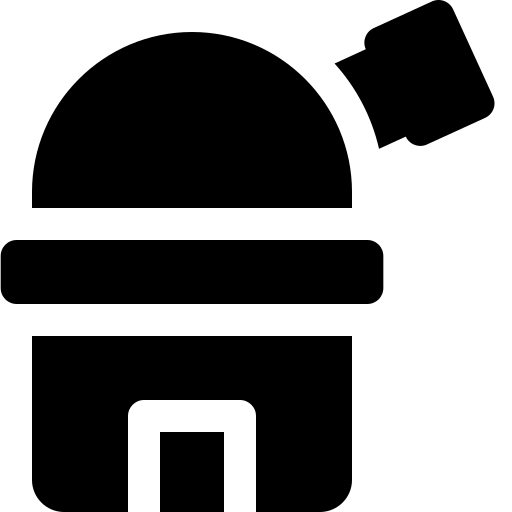
\includegraphics[width=\linewidth]{Image/observatory.png}
\end{minipage}
\hfill
\begin{minipage}[t]{0.85\textwidth}
    Observatory icon \cite{flaticon_observatory_icon}
\end{minipage}

\newpage

\bibliographystyle{plain}
\bibliography{references}
\end{document}
